\documentclass{exam}

\usepackage{siunitx} 
\usepackage{graphicx}
\usepackage[fleqn]{amsmath}
\usepackage{cancel}
\usepackage{float}
\usepackage{mdwlist}
\usepackage{booktabs}
\usepackage{cancel}
\usepackage{polynom}
\usepackage{caption}
\usepackage{fullpage}
\usepackage{xfrac}
\usepackage{comment}

\newcommand{\degree}{\ensuremath{^\circ}} 
\everymath{\displaystyle}

% \begin{figure}[H]
%   \centering
%   \includegraphics[scale=.3]{problem7.eps}
%   \caption*{Problem 7}
% \end{figure}

% \begin{tabular}{cc}
% \toprule
% period & amplitude \\
% \midrule
%   $\pi$ & $2$ \\
% \bottomrule
% \end{tabular}

\excludecomment{comment}

\printanswers

\ifprintanswers 
  \usepackage{2in1, lscape} 
\fi

\author{}
\date{January 16, 2013}
\title{Math 141 \\ Homework Two}

\begin{document}

\maketitle

\section{Homework}

\begin{itemize*}
  \item Read section 2.2 and section 2.3
  \item Section 2.2: 4, 8-9, 11, 14, 17, 20, 23-25, 44, 48, 55-56, 61, 63, 68-69, 83, 85, 87, 91
  \item Section 2.3: 1-4, 13-14, 19-20, 27-34
\end{itemize*}

\section{Extra Credit}
Section 2.3, problems 38 and 39.

\ifprintanswers
  \begin{description}
    \item[38]
      During the first part of the race, the speeds are increasing and the car
      is accelerating:

        \begin{tabular}{lrrrrr}
          \toprule
          interval     &  1 &  2 &  3 &   4 &   5 \\ 
          speed (ft/s) & 17 & 18 & 63 & 147 & 237 \\
          \bottomrule
        \end{tabular}

      During the later part of the race, the speeds are decreasing and the car
      is decelerating:

        \begin{tabular}{lrrrrr}
          \toprule
          interval     &   1 &   2 &  3 &  4 &  5 \\ 
          speed (ft/s) & 263 & 144 & 91 & 74 & 48 \\
          \bottomrule
        \end{tabular}

      A {\em concave up} graph represents an accelerating car and a {\em concave
      down} graph represents a decelerating car.

    \item[39]
      Variations of $f(x) = \pm 2^{\pm x}$ work for all of these.  
     
      \begin{itemize*}
        \item $2^x$ is always positive and always increasing.  
        \item $2^{-x}$ is always positive and always decreasing.  
        \item $-2^{-x}$ is always negative and always increasing.  
        \item $-2^x$ is always negative and always decreasing.  
      \end{itemize*}

      \begin{figure}[H]
        \centering
        \includegraphics[scale=.3]{section_2.3/problem_39a.eps}
        \caption*{(a) always increasing, $f(x) > 0$: $f(x) = 2^x$}
      \end{figure}

      \begin{figure}[H]
        \centering
        \includegraphics[scale=.3]{section_2.3/problem_39b.eps}
        \caption*{(b) always decreasing, $f(x) > 0$: $f(x) = 2^{-x}$}
      \end{figure}

      \begin{figure}[H]
        \centering
        \includegraphics[scale=.3]{section_2.3/problem_39c.eps}
        \caption*{(c) always increasing, $f(x) < 0$: $f(x) = -2^{-x}$}
      \end{figure}

      \begin{figure}[H]
        \centering
        \includegraphics[scale=.3]{section_2.3/problem_39d.eps}
        \caption*{(d) always decreasing, $f(x) < 0$: $f(x) = -2^x$}
      \end{figure}

  \end{description}

  \pagebreak

  \section{Section 2.2}

  \begin{description}
    \item[4]
      \begin{figure}[H]
        \centering
        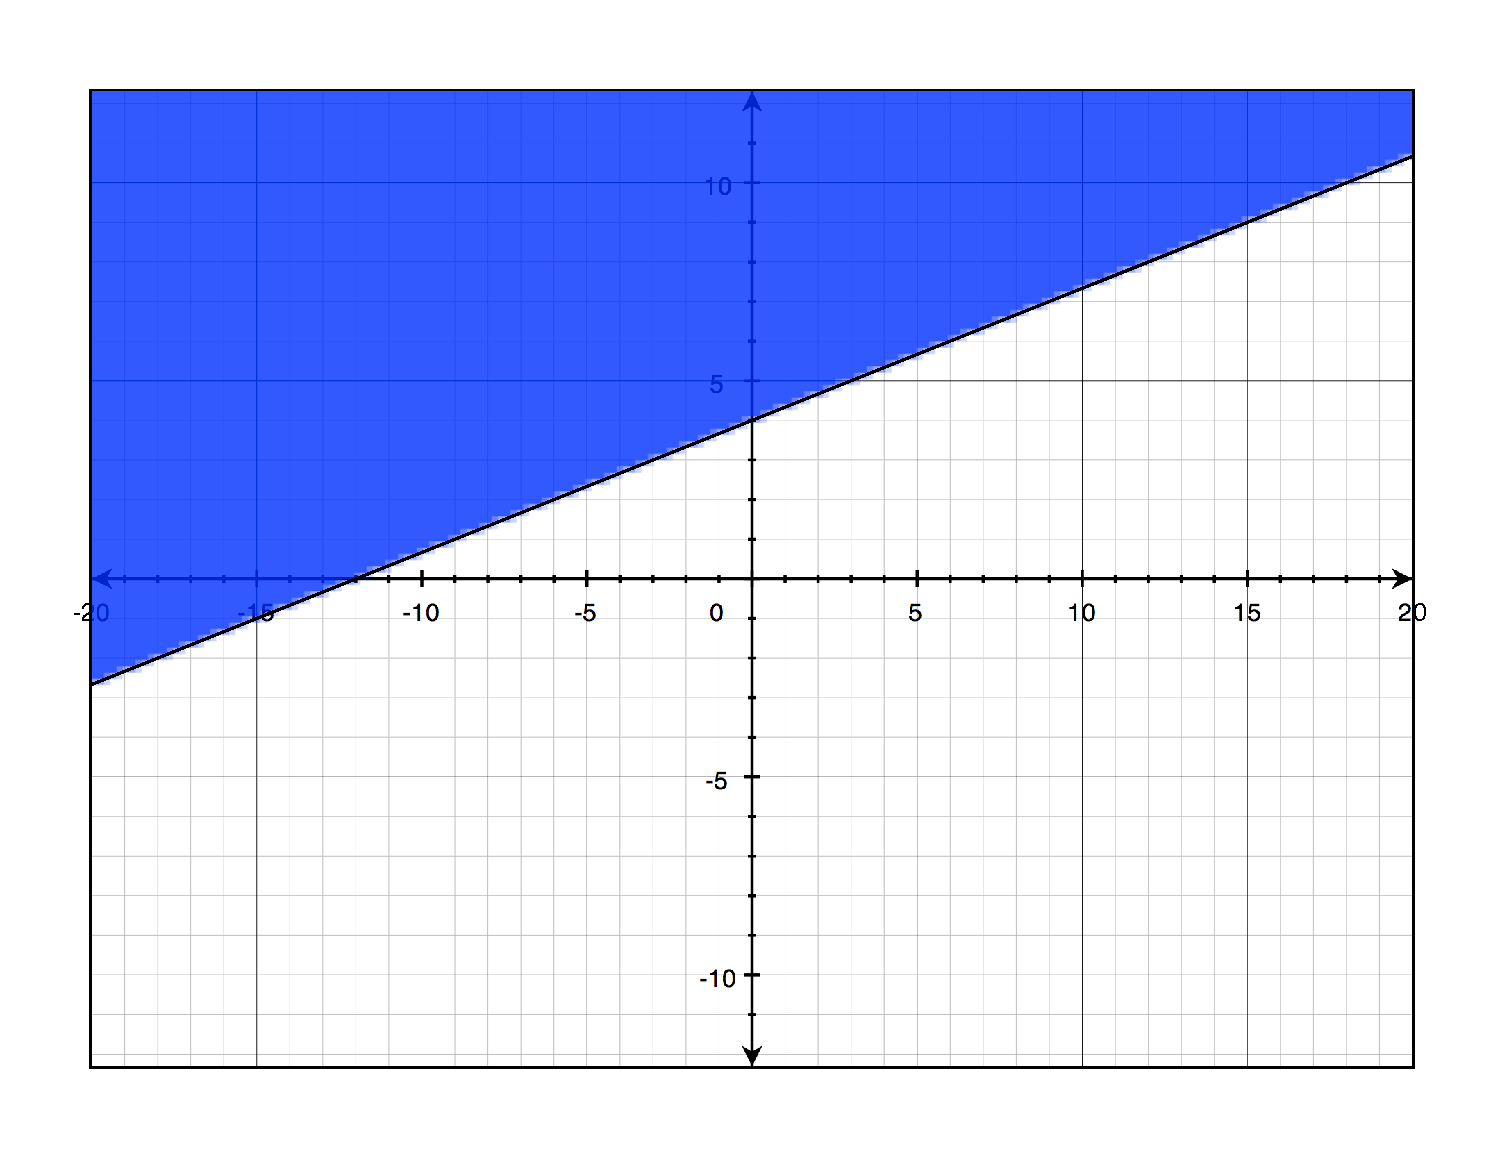
\includegraphics[scale=.3]{section_2.2/problem4.eps}
        \caption*{Problem 4: $y = 6 - 3x$}
      \end{figure}

    \item[8]
      \begin{figure}[H]
        \centering
        \includegraphics[scale=.3]{section_2.2/problem8.eps}
        \caption*{Problem 8: $y = x^2 - 4$}
      \end{figure}

    \item[9]
      \begin{figure}[H]
        \centering
        \includegraphics[scale=.3]{section_2.2/problem9.eps}
        \caption*{Problem 9: $y = x^3 - 4$}
      \end{figure}

    \item[11]
      \begin{figure}[H]
        \centering
        \includegraphics[scale=.3]{section_2.2/problem11.eps}
        \caption*{Problem 11: $y = \sqrt{x + 4}$}
      \end{figure}

    \item[14]
      \begin{figure}[H]
        \centering
        \includegraphics[scale=.3]{section_2.2/problem14.eps}
        \caption*{Problem 14: $y = \frac{1}{x + 4}$}
      \end{figure}

    \item[17]
      \begin{figure}[H]
        \centering
        \includegraphics[scale=.3]{section_2.2/problem17.eps}
        \caption*{Problem 17: $y = |x| + x$}
      \end{figure}

    \item[20]
      \begin{figure}[H]
        \centering
        \includegraphics[scale=.3]{section_2.2/problem20.eps}
        \caption*{Problem 20: $y = \frac{x}{|x|}$}
      \end{figure}

    \item[23].
      
      \begin{parts}
        \part
          \begin{tabular}{lrrrr}
            \toprule
            $x$    & $-2$ & $0$ & $2$ & $3$ \\ 
            $h(x)$ &  $1$ & $-1$ & $3$ & $4$ \\ 
            \bottomrule
          \end{tabular}
        \part
          \begin{itemize*}
            \item domain: $[-3, 4]$
            \item range: $[-1, 4]$
          \end{itemize*}
      \end{parts}

    \item[24].
      
      \begin{parts}
        \part
          \begin{tabular}{lrrrrr}
            \toprule
            $x$    & $-4$ & $-2$ &  $0$ & $2$ & $4$ \\ 
            $g(x)$ &  $3$ &  $2$ & $-2$ & $1$ & $0$ \\ 
            \bottomrule
          \end{tabular}
        \part
          \begin{itemize*}
            \item domain: $[-4, 4]$
            \item range: $[-2, 3]$
          \end{itemize*}
      \end{parts}

    \item[25]
      \begin{parts}
        \part $f(0) > g(0)$
        \part $f(-3) < g(-3)$
        \part $f(-2) = g(-2)$ and $f(2) = g(2)$ 
      \end{parts}

    \item[44]
      \begin{figure}[H]
        \centering
        \includegraphics[scale=.3]{section_2.2/problem44.eps}
        \caption*{Problem 44}
      \end{figure}

    \item[48]
      \begin{figure}[H]
        \centering
        \includegraphics[scale=.3]{section_2.2/problem48.eps}
        \caption*{Problem 48}
      \end{figure}

    \item[55]
      \begin{parts}
        \part function
        \part not a function
        \part function
        \part not a function
      \end{parts}

    \item[56]
      \begin{parts}
        \part not a function
        \part function
        \part function
        \part not a function
      \end{parts}

    \item[61]
      \begin{align*}
        x^2 + 2y &= 4 \\
        2y &= 4 - x^2 \\
        y &= 2 - \frac{x^2}{2} \\
      \end{align*}
      This is a function, since there is only one $y$ value for each $x$ value.

    \item[63]
      \begin{align*}
        x &= y^2 \\
        y &= \pm \sqrt{x} \\
      \end{align*}
      This is not a function, since there are two $y$ values for each $x$ value.

    \item[68]
      \begin{align*}
        \sqrt{x} + y &= 12 \\
        y &= 12 - \sqrt{x} \\
      \end{align*}
      This is a function, since there is only one $y$ value for each $x$ value.

    \item[69]
      \begin{align*}
        x &= y^3 \\
        y &= \sqrt[3]{x} \\
      \end{align*}
      This is a function, since there is only one $y$ value for each $x$ value.

    \item[83]
      The person gained weight steadily until he was 30 when he went on an
      expedition to Antarctica and lost 30 pounds because he had to subsist on a
      diet of penguins for two years.  When he returned to civilization, his
      weight continued its upward trend until he died of a heart attack at age
      67.

    \item[85]
      Hurdler B was the favorite, but unfortunately he neglected to tie his shoe
      before the start of the race.  He jumped out to an early lead, but crashed
      to the ground when his shoelace got tangled with the second hurdle.  It
      took him a few seconds to get to his feet, and by this time it was too
      late for him to catch A, although he was able to pass C.  C meandered
      slowly and steadily to the finish line and finished last.      

    \item[87]
      \begin{parts}
        \part $t = \SI{5}{s}$
        \part $t = \SI{30}{s}$
        \part $t = \SI{17}{s}$
      \end{parts}

    \item[91]
      When $n$ is even, each $y$ value corresponds to two $x$ values, so
      equations with even $n$ are not graphs of functions.  When $n$ is odd,
      each $y$ value corresponds to exactly one $x$ value, so equations with odd
      $n$ are graphs of functions.

  \end{description}

  \pagebreak

  \section{Section 2.3}

  \begin{description}

    \item[1] increasing: $[-1, 1]$, $[2, 4]$; decreasing: $[1, 2]$

    \item[2] increasing: $[0, 1]$; decreasing: $[-2, 0]$, $[1, 3]$ 

    \item[3] increasing: $[-2, -1]$, $[1, 2]$; decreasing: $[-3, -2]$, $[-1, 1]$, $[2, 3]$ 

    \item[4] increasing: $[-1, 1]$; decreasing: $[-2, -1]$, $[1, 2]$ 

    \item[13]
      \[
        \frac{\Delta y}{\Delta x} = \frac{5 - 3}{4 - 1} = \frac{2}{3}
      \]

    \item[14]
      \[
        \frac{\Delta y}{\Delta x} = \frac{2 - 4}{5 - 1} = -\frac{1}{2}
      \]

    \item[19]
      \[
        \frac{\Delta y}{\Delta x} = \frac{24 - (-1)}{4 - (-1)} = 5
      \]

    \item[20]
      \[
        \frac{\Delta y}{\Delta x} = \frac{1 - (-11)}{0 - (-2)} = 6
      \]

    \item[27]
      \begin{align*}
        \frac{\Delta y}{\Delta x} &= \frac{\left( \cfrac{2}{a + h} - \cfrac{2}{a} \right)}{a + h - a} \\
          &= \frac{2a - 2(a + h)}{ah(a + h)} \\
          &= \frac{-2}{a(a + h)} \\
      \end{align*}

    \item[28]
      \begin{align*}
        \frac{\Delta y}{\Delta x} &= \frac{\sqrt{a + h} - \sqrt{a}}{a + h - a} \\
          &= \frac{\sqrt{a + h} - \sqrt{a}}{h} \\
      \end{align*}

    \item[29]
      \begin{parts}
        \part 
          \begin{align*}
             \frac{\Delta y}{\Delta x} &= \frac{\left( \cfrac{a + h}{2} + 3 -
                 \left( \cfrac{a}{2} + 3 \right) \right)}{a + h - a} \\
               &= \frac{\left( \cfrac{a + h}{2} - \cfrac{a}{2} \right)}{h} \\
               &= \frac{a + h - a}{2h} \\
               &= \frac{1}{2} \\
          \end{align*}

        \part
          The average rate of change is always $\sfrac{1}{2}$ which is the same as the line's slope.
      \end{parts}

    \item[30]
      \begin{parts}
        \part 
          \begin{align*}
            \frac{\Delta y}{\Delta x} &= \frac{-4(a + h) + 2 - (-4a + 2)}{a + h - a} \\
              &= \frac{-4a - 4h + 2 + 4a - 2)}{h} \\
              &= \frac{-4h}{h} \\
              &= -4 \\
          \end{align*}

        \part
          The average rate of change is always $-4$ which is the same as the line's slope.
      \end{parts}

  \pagebreak

    \item[31]
      \begin{parts}
        \part $W$ is increasing on days 0-150 and 300-365 and decreasing on days 150-300.
        \part
          \[
            \frac{\Delta y}{\Delta x} = \frac{50 - 75}{200 - 100} = - \frac{1}{4} \text{ ft/day }
          \]
      \end{parts}

    \item[32]
      \begin{parts}
        \part The population is increasing between 1950 and 1975 and decreasing
        after 1975.

        \part The population was the same in 1970 and 1990, so the average rate
        of change for these years was zero.

        \part Over that 20 year period, the number of people leaving or dieing
        was the same as the number of people moving in or being born.
      \end{parts}

    \item[33]
      \begin{parts}
        \part
          \[
            \frac{\Delta y}{\Delta x} = \frac{1591 - 856}{2001 - 1998} = 245 \text{ people/year }
          \]
        \part
          \[
            \frac{\Delta y}{\Delta x} = \frac{826 - 1483}{2004 - 2002} = -328 \text{ people/year }
          \]
        \part The population was increasing between 1997 and 2001.
        \part The population was decreasing between 2001 and 2006.
      \end{parts}

    \item[34]
      \begin{parts}
        \part
          \[
            \frac{\Delta y}{\Delta x} = \frac{800 - 400}{152 - 68} \approx \SI{4.8}{\m/\s}
          \]
        \part
          \[
            \frac{\Delta y}{\Delta x} = \frac{1600 - 1200}{412 - 263} \approx \SI{2.7}{\m/\s}
          \]
        \part
          \begin{tabular}{lr}
            \toprule
            lap & speed \\
            \midrule
            1   & 6.25 \\
            2   & 5.55 \\
            3   & 5.00 \\
            4   & 4.54 \\
            5   & 3.92 \\
            6   & 3.33 \\
            7   & 2.78 \\
            8   & 2.60 \\
            \bottomrule
          \end{tabular}

        \part He gets slower and slower with each passing lap.
      \end{parts}

    \pagebreak
  \end{description}
\else
  \vspace{8 cm}
    \begin{quote}
      Personally I'm in favor of democracy, which means that the central
      institutions in the society have to be under popular control. Now, under
      capitalism we can't have democracy by definition. Capitalism is a system in
      which the central institutions of society are in principle under autocratic
      control. Thus, a corporation or an industry is, if we were to think of it in
      political terms, fascist; that is, it has tight control at the top and
      strict obedience has to be established at every level---there's a little
      bargaining, a little give and take, but the line of authority is perfectly
      straightforward. Just as I'm opposed to political fascism, I'm opposed to
      economic fascism. I think that until major institutions of society are under
      the popular control of participants and communities, it's pointless to talk
      about democracy.
    \end{quote}
  \vspace{.2 cm}

  \hspace{1 cm} --Noam Chomsky
\fi

\end{document}

